% =============================================================================
%  Sección 6: Despersonalización o estandarización
% =============================================================================
\section{El Transporte como Espacio}
\label{transporte-espacio}

\subsection{Definición de Espacios}
\label{definicion-espacio}

La comprensión de la infraestructura de movilidad requiere trascender su visión puramente 
logística e ingenieril para adentrarse en la teoría de la producción del espacio. 
El filósofo Henri Lefebvre \cite{lefebvre2013produccion} postula que el espacio no es un 
contenedor material pasivo, sino un producto intrínsecamente social e ideológico. 
Esta premisa es operativizada por el geógrafo Edward Soja \cite{soja1996thirdspace} 
mediante su \termino{Trialéctica del espacio}, una ontología que entrelaza la materialidad, 
la conceptualización y la experiencia vivida para decodificar los entornos urbanos.

Bajo este marco analítico, y apoyados en la geografía crítica de David Harvey 
\cite{harvey2007espacios} y Neil Smith \cite{smith2020desarrollo}, quienes analizan 
cómo el desarrollo desigual y la acumulación de capital dictan la morfología de la ciudad, 
la infraestructura orientada al transporte puede deconstruirse en tres dimensiones espaciales:

\begin{itemize}
    \item \textbf{Primer Espacio (El espacio percibido / material):} Corresponde a las 
            prácticas espaciales y la red física palpable. Es el asfalto, las vías férreas, 
            los vehículos y las estaciones. Siguiendo a Smith y Harvey, este espacio material 
            a menudo refleja un ``arreglo espacial'' (\textit{spatial fix}) diseñado para 
            acelerar la circulación de mercancías y fuerza de trabajo, reproduciendo 
            frecuentemente la segregación socioespacial del tejido urbano.
    
    \item \textbf{Segundo Espacio (El espacio concebido / representaciones del espacio):} Es 
            el espacio de los planificadores, ingenieros, tecnócratas y el Estado. Son los mapas, 
            los presupuestos, los modelos de zonificación y los algoritmos de flujo. Es el 
            discurso dominante que impone un orden racional y estandarizado sobre la infraestructura, 
            muchas veces ignorando las necesidades orgánicas de la población que la habita.
    
    \item \textbf{Tercer Espacio (El espacio vivido / espacios de representación):} Es el espacio 
            de la experiencia cotidiana, la resistencia y el simbolismo. Es el vagón del metro, 
            el paradero del autobús o la cabina del teleférico. Aquí, el usuario se apropia y 
            subvierte la planificación del Segundo Espacio y la materialidad del Primer Espacio, 
            dotando al trayecto de un significado cultural y social propio.
\end{itemize}

Es en la intersección de esta trialéctica donde cobra vital relevancia la perspectiva del urbanismo 
de asociación de Alison y Peter Smithson \cite{smithson1967urban}. Para los Smithson, las vías 
de circulación no son meros conductos de tránsito, sino escenarios supremos de encuentro 
y \textit{colisión de interacciones espaciales}. El sistema de transporte público es, por 
excelencia, la infraestructura donde el sujeto se ve obligado a interactuar con la otredad. 
En la cápsula espacio-temporal de un vagón o una estación colisionan individuos de distintos 
estratos socioeconómicos, bagajes culturales, edades y etnias. Por lo tanto, dignificar, invertir 
y reforzar el espacio público del transporte no es solamente una medida de eficiencia técnica, sino 
un imperativo sociológico fundamental para construir una sociedad civil más resiliente, empática 
y tolerante ante las profundas diferencias y los inminentes retos urbanos del siglo XXI.

\subsection{Contornos y Periferias}
\label{contornos-periferias}

La \zmvm no puede entenderse como un espacio uniforme, equitativo y resilente en todas sus áreas, 
ni siquiera como un espacio con la misma definición de \termino{Cultura}. Esto no es una invención, 
el mismo gobierno federal lo sabe, y ha creado una delimitación bastante clara entre cada sección 
llamándola así mismo contornos urbanos que se describen en la siguiente frase e imagen: 

\citaclave{
``  Otro nivel de complejidad se debe a que los servicios que conforman el sistema de
    movilidad no fueron diseñados de origen para integrar una red física de transporte
    para la Ciudad de México, ni menos aún, para dar servicio a la Zona Metropolitana
    del Valle de México. Por lo anterior, su integración es uno de los puntos prioritarios
    a atender con el fin de garantizar un servicio de movilidad integrado, digno e
    incluyente.''
  \citep{semovi2020diagnostico}
}

\begin{figure}[htbp]
    \centering
    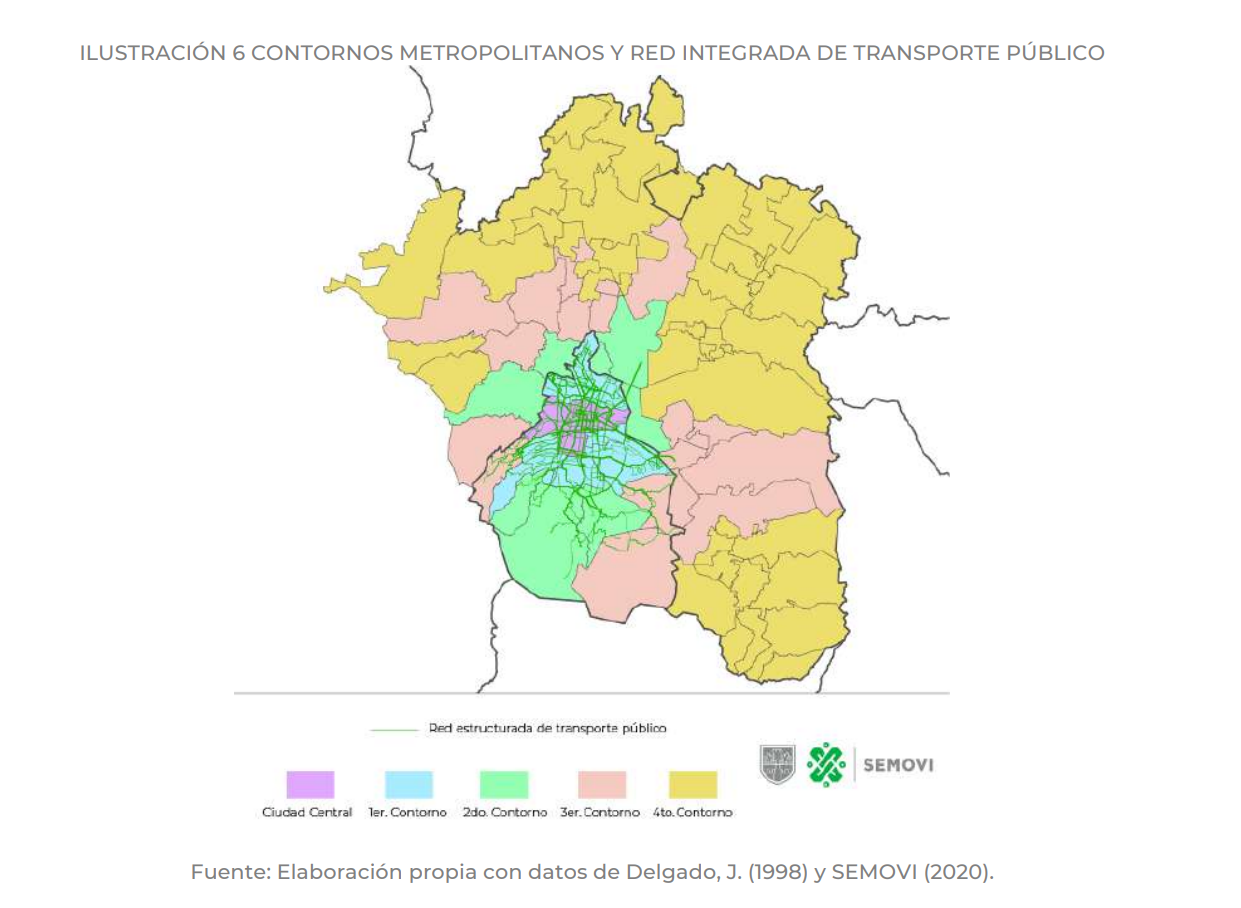
\includegraphics[width=0.80\textwidth]{img/SEMOVITC.png}
    \caption[Contornos Metropolitanos]{Contornos Metropolitanos y red de transporte
    público integrada.}
    \label{fig:semovi-contornos}
    \small\textit{Fuente: Diagnóstico Técnico de Movilidad para el Programa Integral de
    Movilidad (2019--2024, p.~16).}
\end{figure}